%%% Laboratory	 Notes
%%% Template by Mikhail Klassen, April 2013
%%% Contributions from Sarah Mount, May 2014
\documentclass[a4paper]{tufte-handout}
\usepackage[portuguese]{babel}

\newcommand{\workingDate}{\textsc{2024/2025}}
\newcommand{\userName}{João Sá Pereira}
\newcommand{\institution}{FEUP}

\usepackage{lab_notes}

\usepackage{hyperref}
\hypersetup{
    pdffitwindow=false,            % window fit to page
    pdfstartview={Fit},            % fits width of page to window
    pdftitle={Notas Lab 2024-2025},     % document title
    pdfauthor={João Sá Pereira},         % author name
    pdfsubject={},                 % document topic(s)
    pdfnewwindow=true,             % links in new window
    colorlinks=true,               % coloured links, not boxed
    linkcolor=DarkScarletRed,      % colour of internal links
    citecolor=DarkChameleon,       % colour of links to bibliography
    filecolor=DarkPlum,            % colour of file links
    urlcolor=DarkSkyBlue           % colour of external links
}


\title{Notas de Laboratório}
\author{João Sá Pereira}
\date{2024/2025}

\begin{document}
\selectlanguage{portuguese}
\maketitle

%%%%%%%%%%%%%%%%%%%%%%%%%%%%%%%%%%%%%%%%%%%%%%%%%%%%%%%%
\topskip0pt
\vspace*{\fill}
\begin{projects}
	\begin{description}
		\item [INN4MIN] Desenvolvimento de metodologias inovadoras e sustentáveis aplicadas a recuperação de ouro e elementos críticos em minérios e placas de circuito integradas utilizadas\footnote{\href{https://cerena.pt/projects/inn4min-development-innovative-and-sustainable-approaches-applied-recovery-gold-and-1}{ERA-MIN3/0003/2021}}
	\end{description}
\end{projects}

\begin{planos}
    Lixiviação do ouro - Numão (pré-concentrado colhido na mina, cerca de 15~kg)
    \begin{description}
        \item [Preparação de amostras] Amostragens para sacos de 200~g.
        \item [Caracterização da amostra] FRX, Digestão ABS, análise granulométrica $\rightarrow$ fazer em triplicado.
        \item [Lixiviação] Plano de lixiviação com Tioreia (fazer exploratório e depois preparar plano de ensaios)
        \item [Lixiviação] Plano de lixiviação com Citrato.
        \item [Lixiviação] Plano de lixiviação com Bromo.
    \end{description}
    Fazer ensaios exploratórios com os 3 reagentes e, em função dos resultados, preparar plano mais exaustivo.
\end{planos}
\vspace*{\fill}

\pagebreak

%%%%%%%%%%%%%%%%%%%%%%%%%%%%%%%%%%%%%%%%%%%%%%%%%%%%%%%%

% \begin{maybe}
%     \begin{itemize}
%     	\item Reimplement the ideas from the paper \textit{Getting Reference Counting Back in the Ring} \citep{Shahriyar+12}
%     \end{itemize}
% \end{maybe}
%%%%%%%%%%%%%%%%%%%%%%%%%%%%%%%%%%%%%%%%%%%%%%%%%%%%%%%%

\newday{21 Outubro 2024}

Foi feito um trabalho de desagregação da amostra inicial, proveniente da mina do Numão. 
Uma amostra de um pré-concentrado que tinha sido anteriormente submetida a processos de flutuação. 
A amostra tinha cerca de 15~kg.

Foi utilizado um moinho\footnote{\href{https://www.retsch.pt/pt/produtos/trituracao/moinhos-planetarios-e-de-bolas/tm-300/}{Moinho de Tambor TM 300 Retsch}} de bolas com a seguinte configuração de trabalho\footnote{Como o moinho nunca tinha sido utilizado para desagregar amostras, fez-se testes para determinar o tempo necessário de funcionamento e para determinar também a necessidade ou não de bolas.}:
\begin{itemize}
    \item[-] 60 rpm;
    \item[-] Duração de trabalho 30~minutos;
    \item[-] Sentido de rotação inverte de 5 em 5~minutos;
    \item[-] Pausa de 1~minuto entre cada inversão de sentido;
    \item[-] 3,41~kg de bolas.
\end{itemize}


Foi-se colocando partes da amostra dentro do tambor do moinho e deixou-se a desagregar durante o tempo estipulado. 
Uma vez terminado o tempo de funcionamento do moinho, peneirou-se o material desagregado com um peneiro de malha \#1.18~mm\footnote{O peneiro de \#1.18~mm foi utilizado como redundância, apenas para ter a certeza que toda a amostra estava desagregada.}.
Foi-se fazendo este procedimento sucessivamente.

Deixou-se material para o dia seguinte.

\hrulefill

%%%%%%%%%%%%%%%%%%%%%%%%%%%%%%%%%%%%%%%%%%%%%%%%%%%%%%%%

\newday{22 Outubro 2024}

Do dia anterior verificou-se que ainda havia alguns ``blocos'', portanto meteu-se o moinho a trabalhar durante cerca de 15~minutos para desagregar o resto do material.
Quando este terminou, a totalidade da amostra foi desagregada e peneirada com o peneiro \#1.18~mm.

Com o material já desagregado, era necessário agora homogeneizar a amostra.
Para isso, foi utilizado o separador \emph{Jones}\footnote{O separador \emph{Jones}, ou em inglês \emph{riffle splitter}, é utilizado para separar amostras em duas partes quase idênticas.} (esquartelador).
Separou-se a amostra de $\approx$~15~kg em duas amostras de $\approx$~7,5~kg cada - amostra A e amostra B.

A amostra B vai ser guardada.
Foi armazenada em dois sacos de plástico - B$_1$ = 3,36~kg e B$_2$ = 4,28~kg.

A amostra A será separada em sacos de $\approx$~1~kg posteriormente.

\hrulefill

%%%%%%%%%%%%%%%%%%%%%%%%%%%%%%%%%%%%%%%%%%%%%%%%%%%%%%%%
\pagebreak

\newday{24 Outubro 2024}

\textit{N.B.: Anteriormente tinha sido feito uma separação manual. Esta abordagem não poderia estar mais errada, separar a amostra manualmente introduz erros significativos, especialmente em amostras com partículas de diferentes calibres. O Jones é uma das formas representativas e precisas que se utiliza na divisão de amostras.}

\section*{Funcionamento do separador jones} 

O \emph{Jones} separa uma amostra em duas metades, sendo que uma das metades separadas é descartada e trabalha-se com a outra. 

Um esquema de funcionamento desta separação está apresentado na Figura~\ref{fig:diagrama_jones}.

\begin{figure}[!ht]
\centering
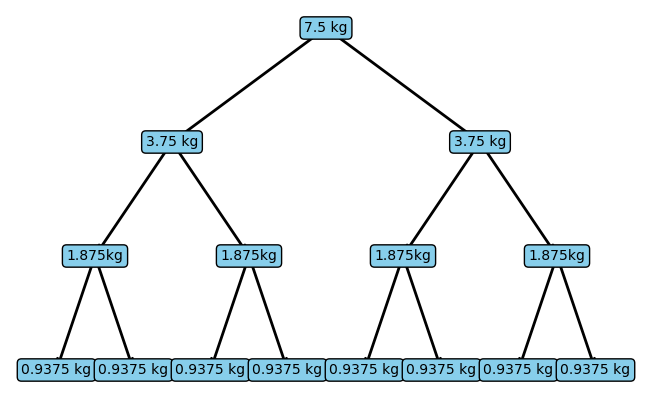
\includegraphics[width=0.9\textwidth]{figures/diagrama_jones.png}
\caption{Diagrama de separação de amostras com o Jones.}
\label{fig:diagrama_jones}
\end{figure}

\hrulefill

%%%%%%%%%%%%%%%%%%%%%%%%%%%%%%%%%%%%%%%%%%%%%%%%%%%%%%%%

\newday{Jan 20 2013}

\textit{N.B.: The following is a sample entry from Mikhail Klassen's research diary. It is intended to be illustrative of how WriteLaTeX can be used the keep track of your research progress. Some names have been removed from this document for privacy.}

\section*{Initial conditions for the turbulent molecular cloud run}

\subsection*{Inner radius}

The density profile follows an $r^{-3/2}$ power law. To avoid a singularity at the center, an interpolation is done over a radius. This inner radius is defined in the parameter file. It should follow the prescription of a singular isothermal sphere (see Binney \& Tremaine p.305), which is also the definition of the King radius:
\begin{equation}
r_0 \equiv \sqrt{\frac{9\sigma^2}{4\pi G\rho_0}}
\end{equation}
where $\sigma$ is the velocity dispersion and could be estimated as $\sigma = \mathcal{M} c_s$, where $c_s = \sqrt{\gamma P/\rho} = \sqrt{\gamma k_B T / \mu}$ is the sound speed.

The isothermal sound speed in our simulation was estimated
\begin{equation}
c_s = \sqrt{\frac{k_b T}{\mu m_p}}
\end{equation}
I'm unsure why a factor of $\gamma$ was not included. For 30 K, this gives a sound speed of about 34000 cm/s or 0.34 km/s. At a Mach number of 5, this gives a supersonic dispersion of $\sigma$ = 1.7 km/s

This gives an inner radius of $r_0 \approx$ 1.595e17. 

\subsection*{Rotation}

Set the same ratio of rotational to gravitational energy $\beta$ as in Peters et al. 2010a. According to Goodman et al. (1993), this is given by (see equation 6):
\begin{equation}
\beta = \frac{1}{4 \pi G \rho_0} \omega^2
\end{equation}
In practice we can probably use the central density $\rho_c$ instead of determining an average density $\rho_0$. Looking at the numbers from other simulations, we could use an $\omega$ of 1.3e-14.

The link to the Goodman et al. (1993) paper:\\
{\tt http://adsabs.harvard.edu/cgi-bin/bib\_query?1993ApJ...406..528G}

We want to complete our simulation with a similar $\beta$ to check if disks form in the turbulent environment.

The $\omega$ necessary to produce a $\beta = 0.05$ would be
\begin{equation}
\omega = \sqrt{4 \pi G \rho_0 \beta} \approx 7.15\times 10^{-13}
\end{equation}
using $\rho_0 = \rho_c = 1.22\times10^{-17}$.

After testing this, however, I found that the rotation was much too fast. Perhaps using $\rho_0 = \rho_c$ was not a very good assumption at all, since $\rho_c$ is orders of magnitude larger than the average. I wrote a little Python script that sums up all the mass inside the outer radius and divides it by the total volume, defined by the outer radius. In this case, for an outer radius of $5.97402\times 10^{18}$ cm and about 1000 $\Msun$, we get an average density of $2.96415\times 10^{-21}$ g/cm$^3$, which gives us $\omega = 1.114 \times 10^{-14}$.

%\hrulefill

%%%%%%%%%%%%%%%%%%%%%%%%%%%%%%%%%%%%%%%%%%%%%%%%%%%%%%%%

%\newpage
\bibliographystyle{plain}
\bibliography{lab_notes}

\end{document}